\section{Case Study}
\label{sec:application}

In this section, we present case studies demonstrating the use of our project. One complex example is highlighted to showcase the correctness and effectiveness of our application. We present more examples that can also be executed directly using our application. In application, you can also hover the mouse on each node for more infomation.

\newpage

\begin{lstlisting}
SELECT
    n_name,
    SUM(l_extendedprice * (1 - l_discount)) AS revenue
FROM
    customer,
    orders,
    lineitem,
    supplier,
    nation,
    region
WHERE
    c_custkey = o_custkey
    AND l_orderkey = o_orderkey
    AND l_suppkey = s_suppkey
    AND c_nationkey = s_nationkey
    AND s_nationkey = n_nationkey
    AND n_regionkey = r_regionkey
    AND r_name = 'ASIA'
    AND o_orderdate >= '1994-01-01'
    AND o_orderdate < '1995-01-01'
    AND c_acctbal > 10
    AND s_acctbal > 20
GROUP BY
    n_name
ORDER BY
    revenue DESC;
\end{lstlisting}

\begin{figure}[ht]
    \centering
    \begin{subfigure}[b]{0.49\linewidth}
        \centering
        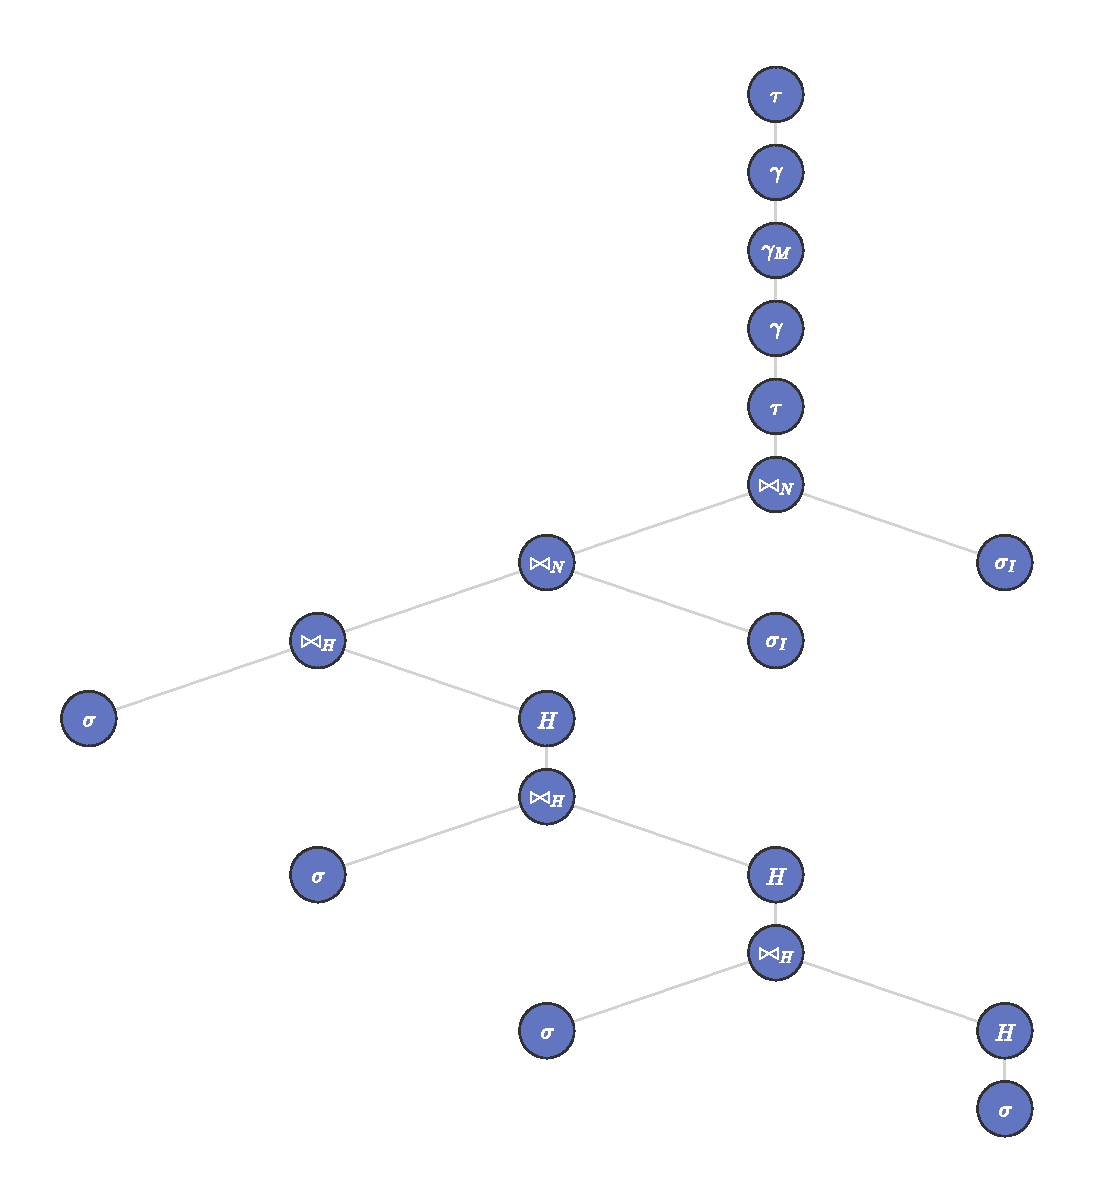
\includegraphics[width=\linewidth]{figures/example1_query_plan.pdf}
        \caption{The visualization of the example query plan using the default settings. The database can freely choose to use which scan type or join type.}
        \label{fig:vis-example-default}
    \end{subfigure}
    \hfill
    \begin{subfigure}[b]{0.49\linewidth}
        \centering
        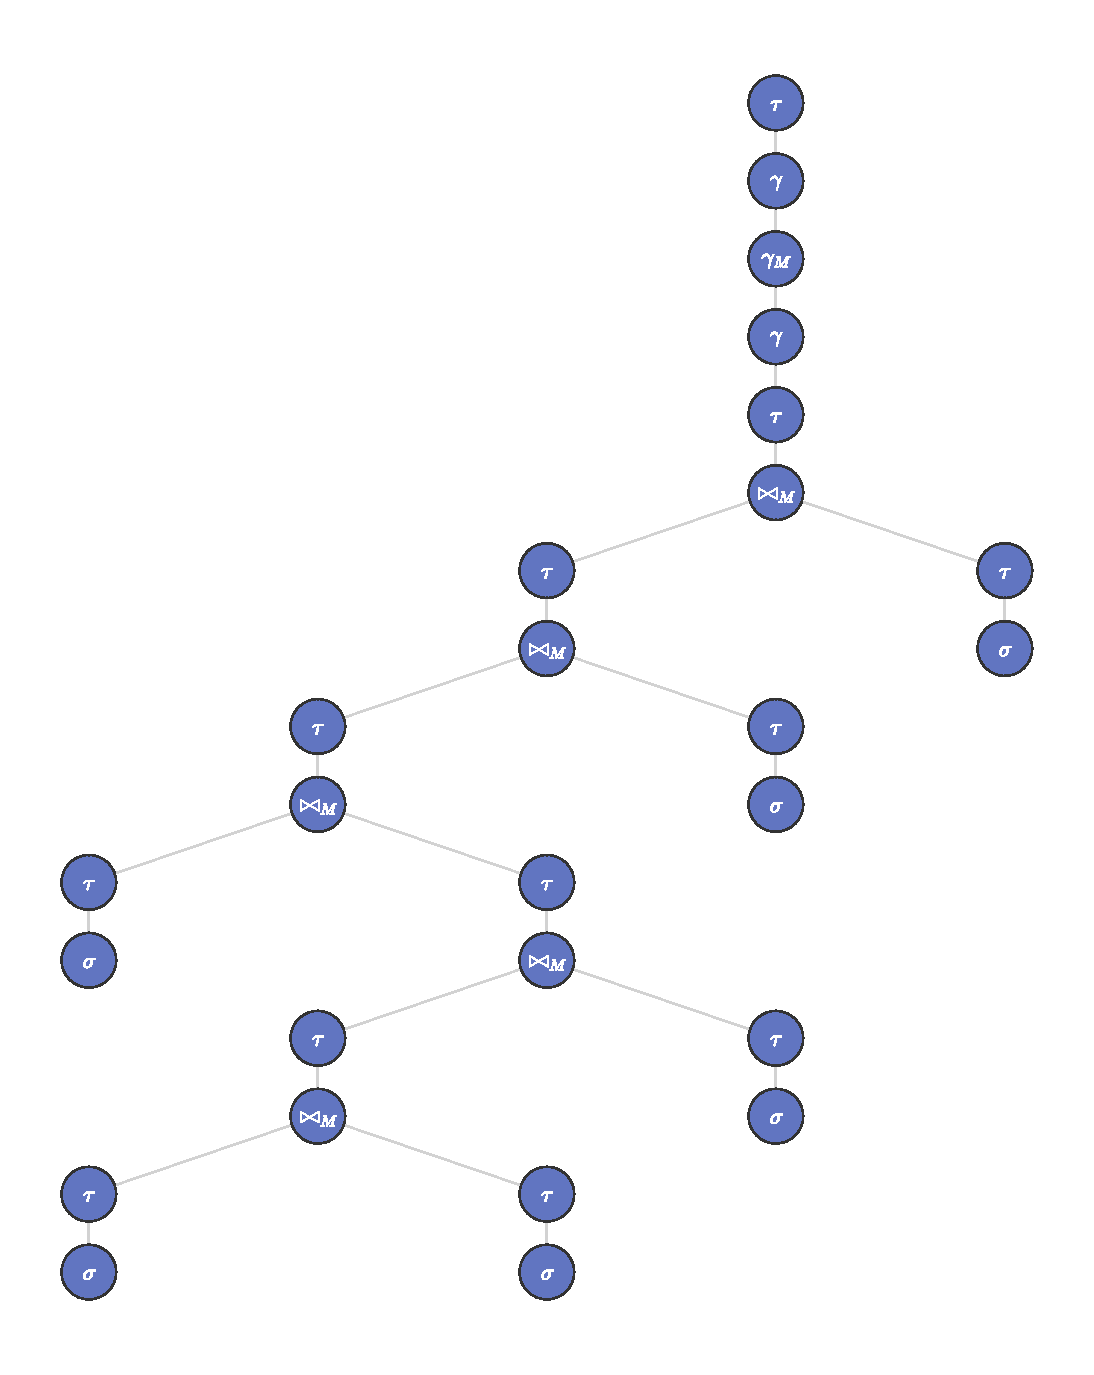
\includegraphics[width=\linewidth]{figures/example1_query_plan_seq_mj.pdf}
        \caption{The visualization of the example query plan by setting the scan method to Sequential Scan and join method to Merge Join.}
        \label{fig:vis-example-ss-mj}
    \end{subfigure}
    \caption{Comparison of the example query plan visualizations.}
    \label{fig:vis-example-comparison}
\end{figure}

\begin{table}[h]
\centering
\begin{tabular}{lll}
\toprule
         & Startup Cost & Total Cost \\
\midrule
Original & 815194.52    & 1434838.82 \\
Revised  & 6592161.29   & 6813958.6 \\
\bottomrule
\end{tabular}
\label{tab:cost-comp}
\caption{The estimated cost for different QEP}
\end{table}

\paragraph{QEP and AQP comparisons} The original Query Execution Plan (QEP) for the above case study example uses scanning method of Index Scan and Sequential Scan to perform selecting; it also performs join using Nested Loop Join and Hash Join; the QEP is shown in~\cref{fig:vis-example-default}. Then the user tests the changes that can be caused by modifying scan method to Sequential Scan and join method to Nested Loop Join, which generates an AQP; the AQP is shown in~\cref{fig:vis-example-ss-mj}. As observed from the above graphs for query plans, the AQP is different from the initial QEP in tree structure and operator sequences. The revised QEP is forced to use sequential scan and merge join for each of the node. We show their estimation cost in~\cref{tab:cost-comp}.

